\documentclass[10pt]{article}


%\topmargin=0cm
\topmargin=-2cm
\addtolength{\textheight}{6.5cm}
\addtolength{\textwidth}{2.0cm}
\usepackage{graphicx}
\usepackage{float}

\begin{document}

\section*{Student Information } 
Full Name : Yavuz Selim Yesilyurt \\
Id Number : 2259166 \\

\section*{Answer 1}
\hspace{4mm}	
IP numbers of the interfaces of attacker, victim, user to OVS are; 10.10.2.2, 10.10.1.1 and 10.10.3.2 respectively. Ip numbers of the interfaces of OVS machines are; 10.10.3.1 (interface to user), 10.10.1.2 (interface to victim) and 10.10.2.1 (interface to attacker).

\section*{Answer 2}
\hspace{4mm}	
Because ICMP is a Network Layer protocol and it is established between host to host; not between process to process. Since it is not established between process to process it doesn't need a port number on either side.

\section*{Answer 3}
\hspace{4mm}	
   Wireshark sequence numbers of first 5 request packets with their corresponding reply  packets are: \\
\begin{center}
12 $->$ no reply packet \\
13 $->$ 14 is the reply packet \\
15 $->$ no reply packet \\
16 $->$ no reply packet \\
17 $->$ 18 is the reply packet \\
\end{center}   

\section*{Answer 4}
\hspace{4mm}	
First ICMP request packet does not have any response so I decided to examine second ICMP request packet. \\

Its wireshark sequence number is 13, ICMP type is 8 (Echo (ping) request), code number is 0, checksum field is 2 bytes, sequence number field is 2 bytes, identifier 2 is bytes. \\

Its reply packet's wireshark sequence number is 14, ICMP type is 0 (Echo (ping) reply), code number is 0, checksum field is 2 bytes, sequence number field is 2 bytes, identifier field is 2 bytes. 

\section*{Answer 5}
\hspace{4mm}	
Following table shows TTL values of packets by means of source-destination address pairs: \\

\begin{table}[H]
\small
\centering
\begin{tabular}{|c|c|}	
\hline
Source - Destination & TTL Value\\
\hline 
10.10.2.2 - 10.10.1.1 (1st request-with no reply) & 64 \\	
10.10.2.2 - 10.10.1.1 (2nd request) & 63 \\			
10.10.1.1 - 10.10.2.2 (1st reply) & 64 \\		
10.10.1.1 - 10.10.2.2 (2nd reply-with no request) & 63 \\
10.10.3.2 - 10.10.3.1  & 64 \\
10.10.3.1 - 10.10.3.2  & 64 \\
\hline 
\end{tabular}
\end{table}

There seems a problem on ICMP packets betweeen 10.10.2.2 and 10.10.1.1. For every request/reply cluster, 10.10.2.2 interface of attacker sends a request packet with ttl=64, but it gets no response; so it sends another request packet with ttl=63, then it gets response from victim with ttl=64. Afterwards, victim sends another reply packet(seemingly a reply packet for the first request packet of attacker) with ttl=63 but it does not reply any of the request packets from 10.10.2.2. \\

For TTL values, we see that ttl value for the first transmitted packet(request or reply does not matter) is 64 and for each retransmitted ICMP packet ttl values gets decremented by one. For instance, as can be seen in above table, ttl values of retransmitted request packet from 10.10.2.2 and retransmitted reply packet from 10.10.1.1 are 63, whereas in their first transmissions they were 64.

\section*{Answer 6}
\hspace{4mm}	
Screenshot of graphical illustration of resources: 

\begin{figure}[H]
    \centering
    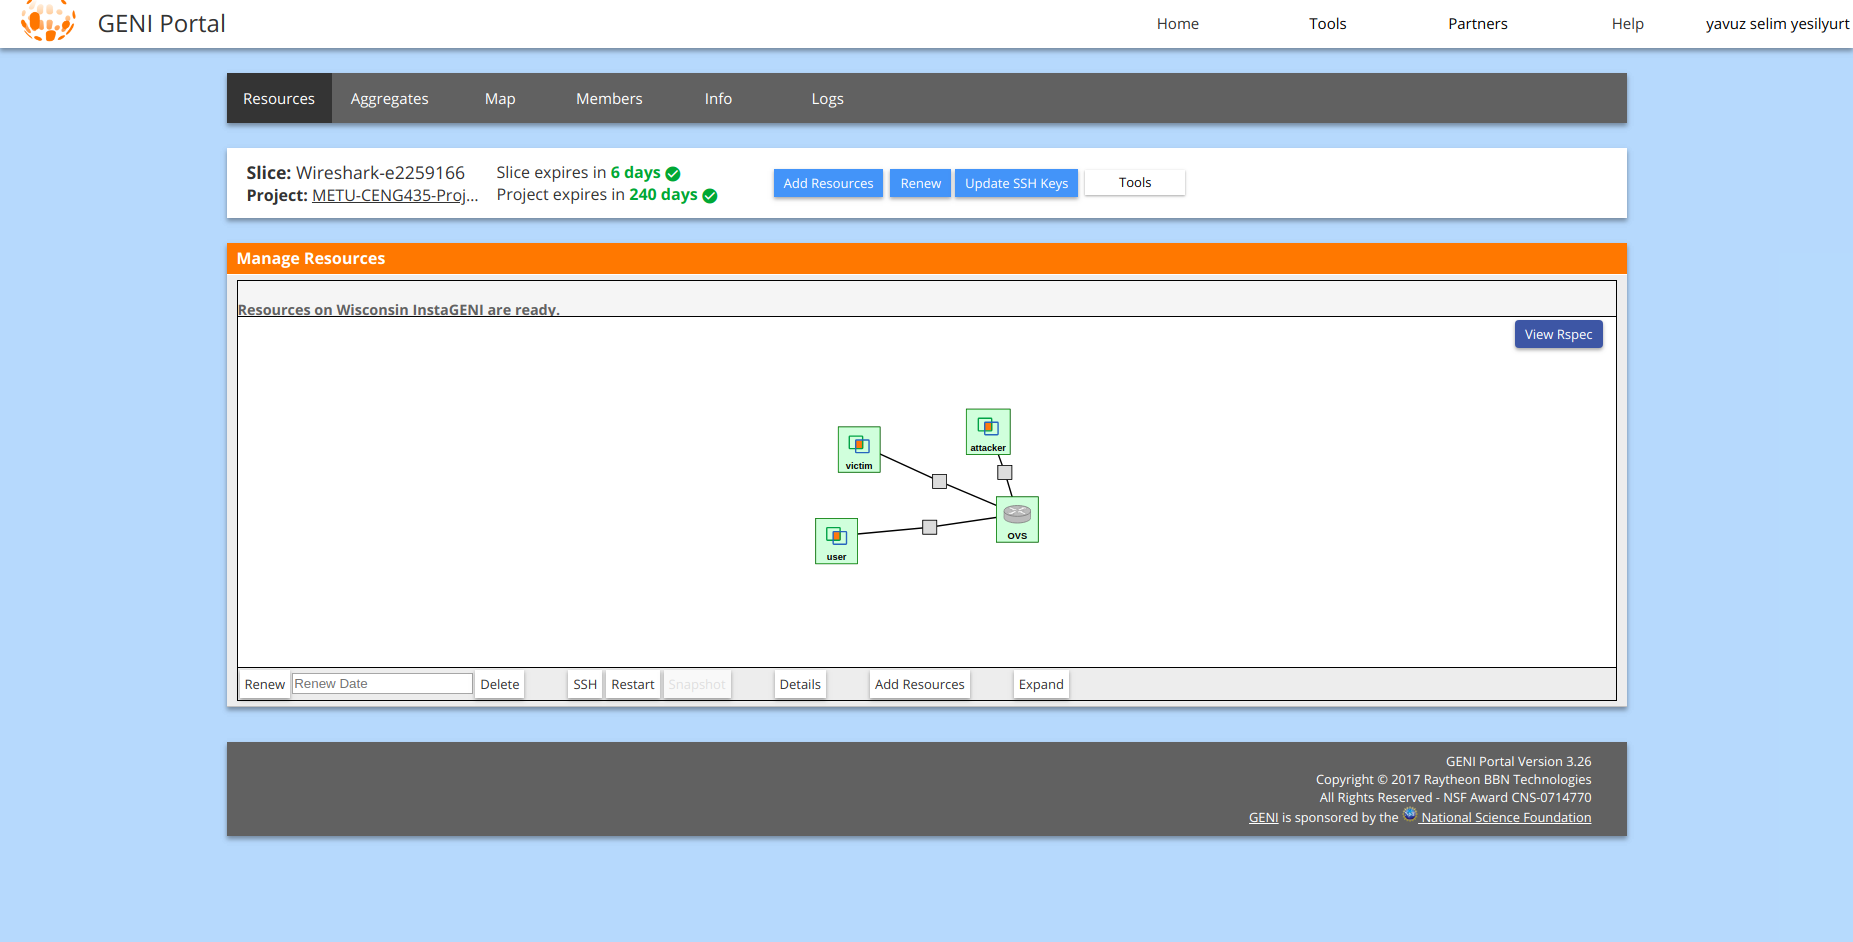
\includegraphics[scale=0.2]{1.png}
\end{figure}

\newpage
Screenshot "details" page: 

\begin{figure}[H]
    \centering
    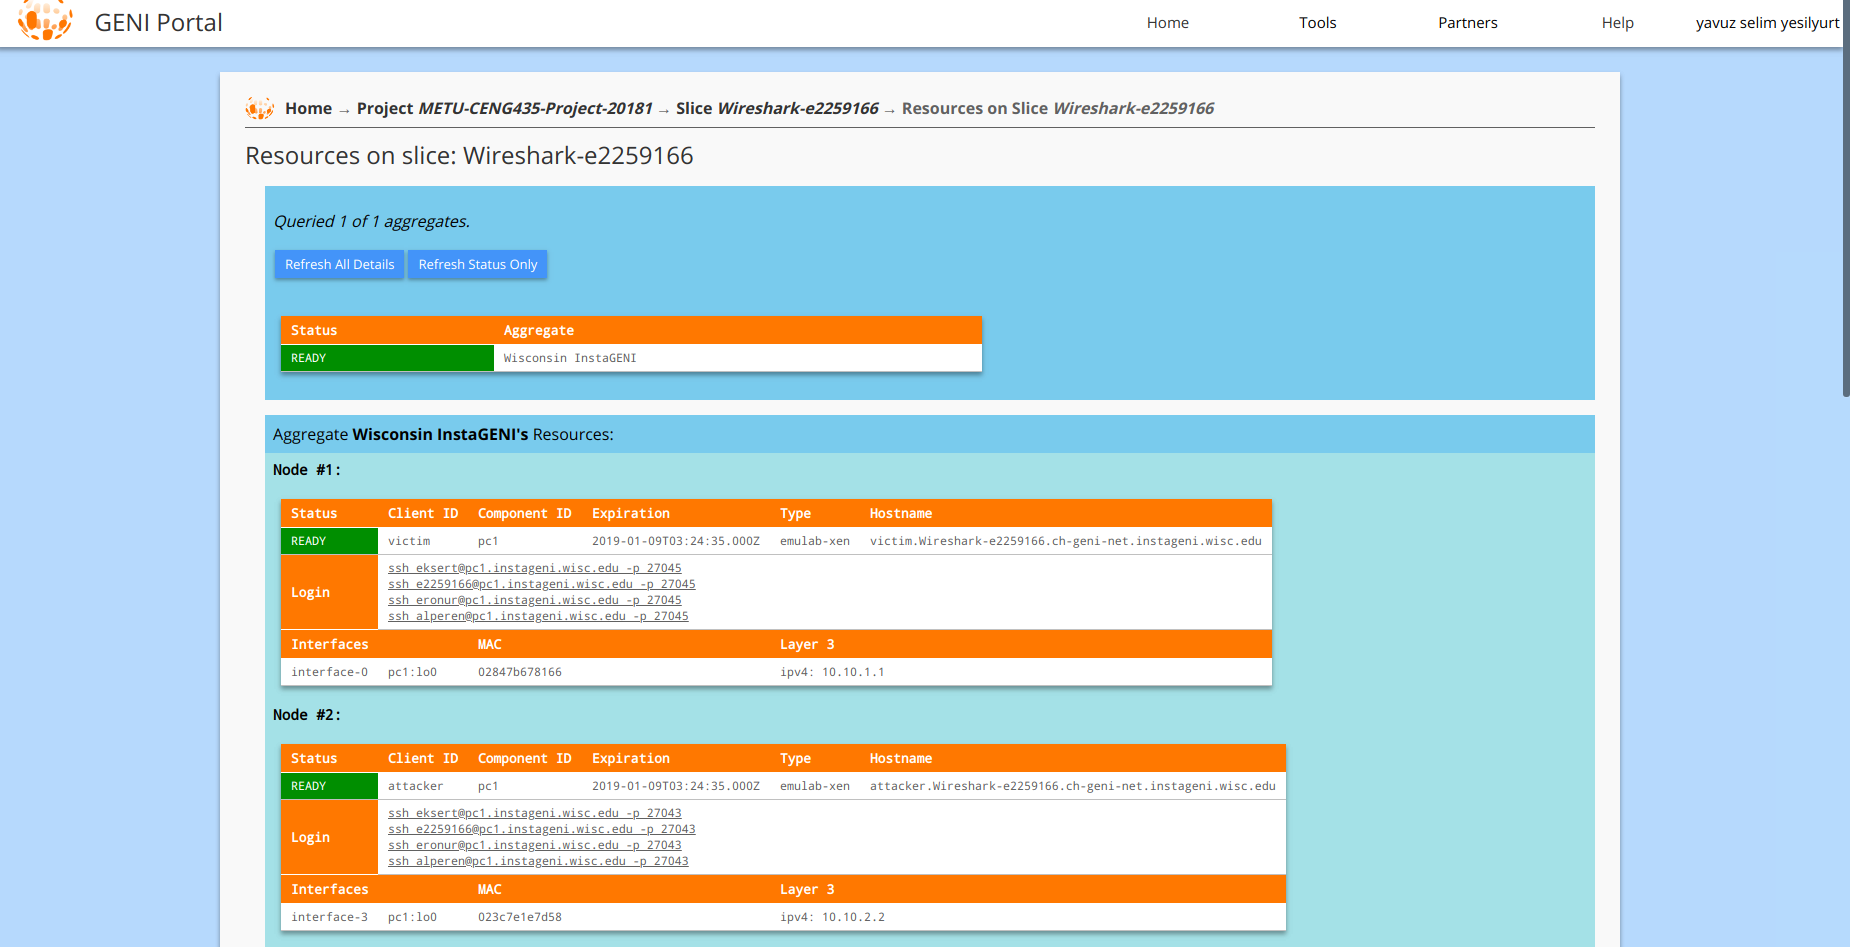
\includegraphics[scale=0.2]{2.png}
    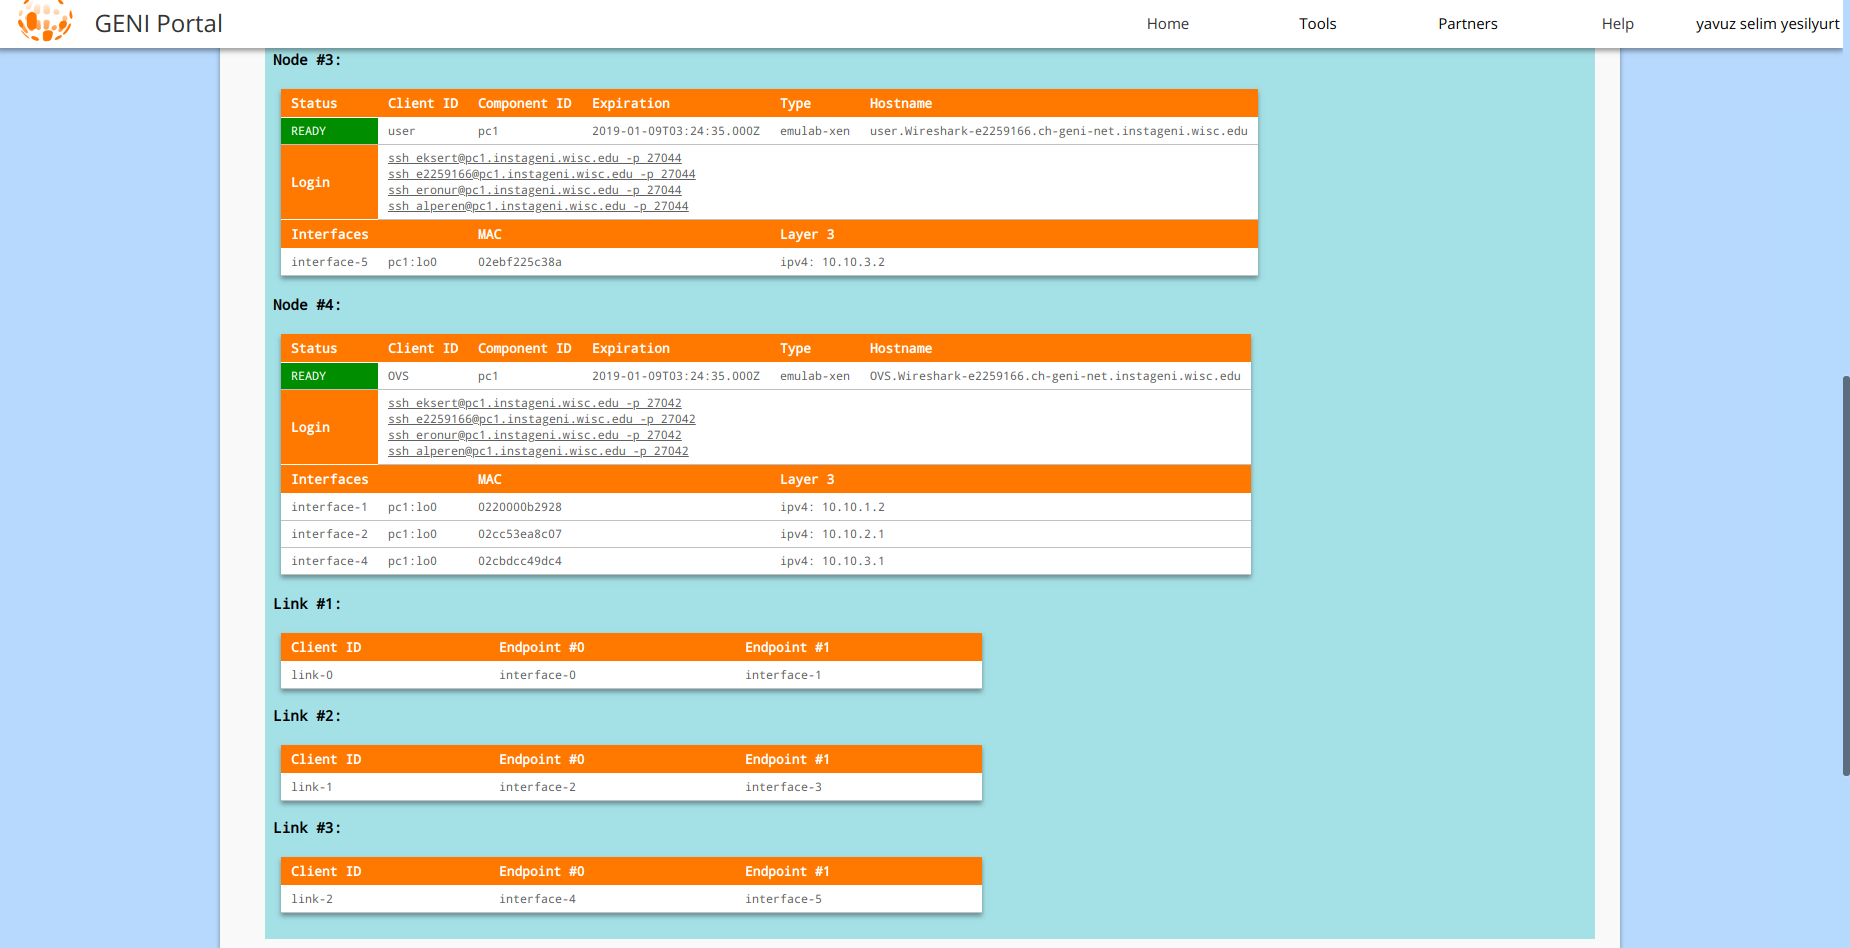
\includegraphics[scale=0.2]{3.png}
\end{figure}


\end{document}

​

